% Copyright (c) 2016 2017 The ALF project.
% This is a part of the ALF project documentation.
% The ALF project documentation by the ALF contributors is licensed
% under a Creative Commons Attribution-ShareAlike 4.0 International License.
% For the licensing details of the documentation see license.CCBYSA.
% !TEX root = doc.tex
\label{sec:kondo}

The Kondo lattice model we consider is an SU(N) generalization of the SU(2) Kondo-model discussed in \cite{Capponi00,Assaad99a}.
Here we follow the work of  Ref.~\cite{Raczkowski20}.
Let $T^{a}$ be the $N^2 -1  $ generators of $SU(N)$ that satisfy the normalization condition: 
\begin{equation}
	\Tr  \left[ T^{a} T^{b} \right]   = \frac{1}{2}\delta_{a,b}.
\label{Normalization_condition.eq}
\end{equation}
For the SU(2) case $T^{a}$  corresponds to the $T  = \frac{1}{2} \ve{\sigma}$ with $\ve{\sigma}$   a vector of the three Pauli spin matrices.      The   Hamiltonian is defined on bilayer  square or honeycomb lattices, with  hopping restricted to the  first layer  (i.e  conduction orbitals $\ve{c}^{\dagger}_{i}  )$   and  spins, f-orbitals, on the second layer. 
\begin{multline}
	\hat{H} = - t  \sum_{\langle i,j \rangle}    \sum_{\sigma=1}^{N}  \left(  \hat{c}^{\dagger}_{i,\sigma}  e^{\frac{2\pi i}{\Phi_0}  \int_{i}^{j} \ve{A}\cdot d \ve{l}}\hat{c}^{\phantom\dagger}_{j,\sigma}   + H.c.  \right)  - \mu \sum_{i,\sigma} \hat{c}^{\dagger}_{i,\sigma}  \hat{c}^{\phantom\dagger}_{i,\sigma}  \\ 
   + \frac{U_c}{N}  \sum_{i}   \left( \hat{n}^c_i -  \frac{N}{2} \right)^2  
         +  \frac{2 J}{N} \sum_{i, a=1  }^{N^2 -1}  \hat{T}^{a,c}_{i}  \hat{T}^{a,f}_{i}. 
\label{Kondo_SUN_Ham.eq}
\end{multline}
In the above, $i$ is a super-index accounting for the unit cell and orbital,
\begin{equation}
	 \hat{T}^{a,c}_{i}   =   \sum_{\sigma,\sigma'=1}^{N} \hat{c}^{\dagger}_{i,\sigma}T^{a}_{\sigma,\sigma'}  \hat{c}^{\phantom\dagger}_{i,\sigma'}, \; \; 
	  \hat{T}^{a,f}_{i}   = \sum_{\sigma,\sigma'=1}^{N} \hat{f}^{\dagger}_{i,\sigma} T^{a}_{\sigma,\sigma'}  \hat{f}^{\phantom\dagger}_{i,\sigma'},  
	  \;\text{ and }\;   \hat{n}^c_i  = \sum_{\sigma=1}^{N} \hat{c}_{i,\sigma}^{\dagger} \hat{c}_{i,\sigma}^{\phantom\dagger} 
\end{equation}
Finally, the constraint
\begin{equation}
   \sum_{\sigma=1}^{N}  \hat{f}^{\dagger}_{i,\sigma}   \hat{f}^{\phantom\dagger}_{i,\sigma}  \equiv  \hat{n}^{f}_i = \frac{N}{2}
\end{equation}
holds. Some rewriting has to be carried out so as to implement  the model.
First, we  use the  relation:
\begin{equation*}
	\sum_{a} T^{a}_{\alpha,\beta} T^{a}_{\alpha',\beta'} = \frac{1}{2} \left(  \delta_{\alpha,\beta'}  \delta_{\alpha',\beta} - \frac{1}{N} \delta_{\alpha,\beta} \delta_{\alpha', \beta'} \right), 
\end{equation*}
to  show that  in the unconstrained Hilbert space,
\begin{align}
	 \frac{2 J}{N} \sum_{ a=1  }^{N^2 -1}  \hat{T}^{a,c}_{i}  \hat{T}^{a,f}_{i}   = &   - \frac{J}{2N} \sum_{i}  \left( 
                \hat{D}^{\dagger}_{i} \hat{D}^{\phantom\dagger}_{i}   +    \hat{D}^{\phantom\dagger}_{i} \hat{D}^{\dagger}_{i}    \right)    + \frac{J}{N}   \left(   \frac{\hat{n}^{c}_i}{2}  + \frac{\hat{n}^{f}_i}{2} -  \frac{\hat{n}^{c}_i \hat{n}^{f}_i}{N}   \right) \nonumber 
 \end{align}
with
\begin{equation*}
	   \hat{D}^{\dagger}_{i}   =  \sum_{\sigma=1}^{N} \hat{c}^{\dagger}_{i,\sigma}  \hat{f}^{\phantom\dagger}_{i,\sigma}.
\end{equation*}
In the constrained Hilbert space, $\hat{n}^{f}_i = N/2 $, the above gives:
\begin{align}
	 \frac{2 J}{N} \sum_{ a=1  }^{N^2 -1}  \hat{T}^{a,c}_{i}  \hat{T}^{a,f}_{i}   =     -  \frac{J}{4N}    \left[ \left(   \hat{D}^{\dagger}_{i}  + \hat{D}^{\phantom\dagger}_{i}    \right)^{2}  + 
                                                       \left(  i\hat{D}^{\dagger}_{i}  - i  \hat{D}^{\phantom\dagger}_{i}    \right)^2  \right] + \frac{J}{4}.  
 \end{align}
The perfect square form complies with the requirements of ALF.
We still have to impose the constraint.
To do so, we work in the unconstrained Hilbert space and add a Hubbard  $U$-term on  the f-orbitals.
With this addition, the Hamiltonian we simulate reads: 

\begin{multline}
	\hat{H}_\textrm{QMC}     =    - t  \sum_{\langle i,j \rangle}    \sum_{\sigma=1}^{N}  \left(  \hat{c}^{\dagger}_{i,\sigma}  e^{\frac{2\pi i}{\Phi_0}  \int_{i}^{j} \ve{A}\cdot d \ve{l}}\hat{c}^{\phantom\dagger}_{j,\sigma}   + H.c.  \right)  - \mu \sum_{i,\sigma} \hat{c}^{\dagger}_{i,\sigma}  \hat{c}^{\phantom\dagger}_{i,\sigma} 
	+    \frac{U_c}{N}  \sum_{i}   \left( \hat{n}^c_i -  \frac{N}{2} \right)^2  \\
    -    \frac{J}{4N}    \left[ \left(   \hat{D}^{\dagger}_{i}  + \hat{D}^{\phantom\dagger}_{i}    \right)^{2}  + 
                                                       \left(  i\hat{D}^{\dagger}_{i}  - i  \hat{D}^{\phantom\dagger}_{i}    \right)^2  \right]  
       +    \frac{U_f}{N}  \sum_{i}   \left( \hat{n}^f_i -  \frac{N}{2} \right)^2.
\label{Kondo_SUN_Ham_QMC.eq}
\end{multline}
The key point for the efficiency of the code, is to  see that 
\begin{equation}
	\left[   \hat{H}_\textrm{QMC},  \left( \hat{n}^f_i -  \frac{N}{2} \right)^2  \right]    = 0 
\label{Constraint_KLM.eq}
\end{equation}
such that the  constraint is implemented  efficiently.  In fact, for the finite temperature code  at inverse temperature $\beta$,  the unphysical Hilbert space   is suppressed by a  
factor  $e^{- \beta U_f/N} $. 





\subsubsection*{ The SU(2) case } 
The SU(2) case is special and allows for a more efficient implementation than  mentioned above.    The  key point is that  for the SU(2) case, the  Hubbard term is  related to  the fermion parity,
\begin{equation} 
   \left(   \hat{n}^f_i - 1 \right)^2    = \frac{  (-1)^{\hat{n}^f_i}  +1 }{2}
\end{equation}
such that we can omit the \textit{current}-term  $ \left(  i\hat{D}^{\dagger}_{i}  - i  \hat{D}^{\phantom\dagger}_{i}    \right)^2 $    without violating  Eq.~\ref{Constraint_KLM.eq}.  
As in Refs.~ \cite{Assaad99a,Capponi00,Beach04}.  
the Hamiltonian that one will simulate reads: 
 \begin{multline}
 \label{eqn:ham_kondo}
 	\hat{\mathcal{H}}  =
	\underbrace{-t \sum_{\langle i,j \rangle,\sigma} \left( \hat{c}_{i,\sigma}^{\dagger} e^{\frac{2\pi i}{\Phi_0}  \int_{i}^{j} \ve{A}\cdot d \ve{l}} \hat{c}_{j,\sigma}^{\phantom\dagger}   + \text{H.c.} \right) +
	  \frac{U_c}{2}   \sum_{i}   \left( \hat{n}^{c}_{i} -1 \right)^2    }_{\equiv \hat{\mathcal{H}}_{tU_c}}  \\
  - \frac{J}{4} 	\sum_{i} \left( \sum_{\sigma} \hat{c}_{i,\sigma}^{\dagger}  \hat{f}_{i,\sigma}^{\phantom\dagger}  + 
	                                                        \hat{f}_{i,\sigma}^{\dagger}  \hat{c}_{i,\sigma}^{\phantom\dagger}   \right)^{2}   +
        \underbrace{\frac{U_f}{2}   \sum_{i}   \left( \hat{n}^{f}_{i} -1 \right)^2}_{\equiv \hat{\mathcal{H}}_{U_f}}.
 \end{multline}
The  relation to the Kondo lattice model follows  from expanding the square  of the hybridization to obtain: 
 \begin{equation}
 	\hat{\mathcal{H}}  =\hat{\mathcal{H}}_{tU_c}   
	+ J \sum_{\vec{i}}  \left(  \hat{\vec{S}}^{c}_{\vec{i}} \cdot  \hat{\vec{S}}^{f}_{\vec{i}}    +   \hat{\eta}^{z,c}_{\vec{i}} \cdot  \hat{\eta}^{z,f}_{\vec{i}}  
		-  \hat{\eta}^{x,c}_{\vec{i}} \cdot  \hat{\eta}^{x,f}_{\vec{i}}  -  \hat{\eta}^{y,c}_{\vec{i}} \cdot  \hat{\eta}^{y,f}_{\vec{i}} \right) 
	 + \hat{\mathcal{H}}_{U_f}.
 \end{equation}
 where the $\eta$-operators  relate to the spin-operators via a particle-hole transformation in one spin sector: 
 \begin{equation} 
 	\hat{\eta}^{\alpha}_{\vec{i}}  = \hat{P}^{-1}  \hat{S}^{\alpha}_{\vec{i}} \hat{P}  	\; \text{ with }  \;   
	\hat{P}^{-1}  \hat{c}^{\phantom\dagger}_{\vec{i},\uparrow} \hat{P}  =   (-1)^{i_x+i_y} \hat{c}^{\dagger}_{\vec{i},\uparrow}  \; \text{ and }  \;   
	\hat{P}^{-1}  \hat{c}^{\phantom\dagger}_{\vec{i},\downarrow} \hat{P}  = \hat{c}^{\phantom\dagger}_{\vec{i},\downarrow} 
 \end{equation}
 Since the $\hat{\eta}^{f} $- and $ \hat{S}^{f} $-operators  do not alter the  parity [$(-1)^{\hat{n}^{f}_{\vec{i}}}$ ] of the $f$-sites, 
 \begin{equation}
 	\left[  \hat{\mathcal{H}}, \hat{\mathcal{H}}_{U_f} \right] = 0.
 \end{equation}
 Thereby,  and for positive values of $U$ ,  doubly occupied  or empty $f$-sites -- corresponding to even parity sites -- are suppressed  by a  Boltzmann factor 
 $e^{-\beta U_f/2} $ in comparison to odd parity sites.   Choosing $\beta U_f $ adequately essentially allows to  restrict the Hilbert space to  odd parity $f$-sites.  
 In this Hilbert space $\hat{\eta}^{x,f} = \hat{\eta}^{y,f} =  \hat{\eta}^{z,f} =0$  such that the Hamiltonian (\ref{eqn:ham_kondo}) reduces to the Kondo lattice model. 

%An implementation of the Kondo Lattice model on the  Honeycomb lattice with additional z-z frustration considered in Ref.~\cite{SatoT17_1}, 
%\begin{equation}
%\hat{H}_{\text{Spin}} = J^{z}\sum_{\langle \langle i,j \rangle \rangle}\hat{S}_{i}^{z}\hat{S}_{j}^{z},  \hfill  \hat{H}_{\text{Fermion}} = -t\sum_{\langle i,j \rangle,\sigma}\hat{c}_{i\sigma}^\dagger \hat{c}^{\phantom\dagger} _{j\sigma},  \hfill
%\hat{H}_{\text{Kondo}}  =  J^{\text{K}} \sum_{i}    \frac{1}{2} \hat{\pmb{c}}^{\dagger}_{i} \pmb{\sigma}\hat{\pmb{c}}^{\phantom\dagger}_{i} \cdot \hat{{\bm S}}^{\phantom\dagger} _{i} , \hfill
%\end{equation}
%can be found in  the \texttt{Hamiltonian\_Kondo\_Honey\_mod.F90}

\subsubsection*{ QMC implementation } 

The name space for this model class  reads: 

\begin{lstlisting}[style=fortran,escapechar=\#,breaklines=true]
&VAR_Kondo                 !! Variables for the Kondo  class
ham_T     = 1.d0            ! Hopping parameter
ham_chem  = 0.d0            ! Chemical potential
ham_Uc    = 0.d0            ! Hubbard interaction  on  c-orbitals Uc
ham_Uf    = 2.d0            ! Hubbard interaction  on  f-orbials  Uf
ham_JK    = 2.d0            ! Kondo Coupling  J
/
\end{lstlisting}

Aside from the usual observables  we have included  the scalar observable \texttt{Constraint\_scal}    that measures 
\begin{equation}
	\left<    \sum_{i}   \left( \hat{n}_i^f - \frac{N}{2} \right)^2 \right>.
\end{equation}
$U_f$ has to be chosen large enough  such that  the above quantity vanishes within statistical uncertainty.  For the square lattice,  Fig.~\ref{Constraint.fig}   plots   the  aforementioned quantity as a function of $U_f$  for the SU(2) model.  As apparent $ \left<    \sum_{i}   \left( \hat{n}_i^f - \frac{N}{2} \right)^2 \right> \propto e^{-\beta U_f/2} $.
\begin{figure}
\center
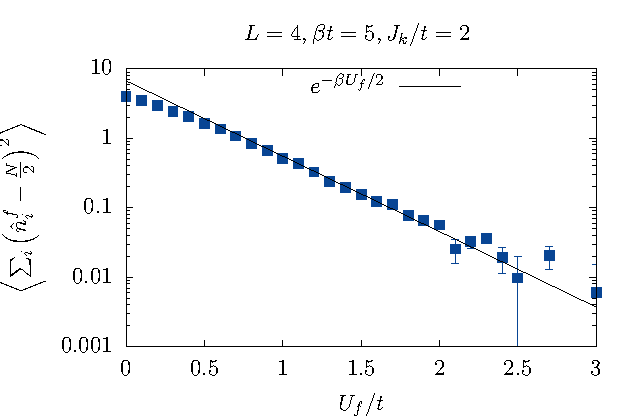
\includegraphics[width=0.49\textwidth]{Figures/Kondo/Constraint.pdf}
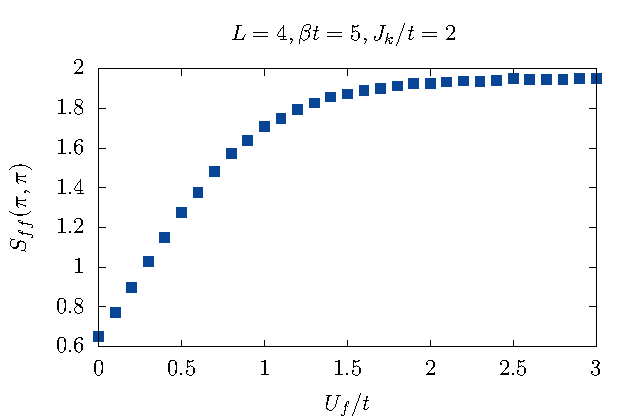
\includegraphics[width=0.49\textwidth]{Figures/Kondo/Spin.pdf}

\caption{Left:  Suppression of charge fluctuations of the f-orbitals as a function of $U_f$.  Right:   When  charge fluctuations  on the f-orbitals vanish, quantities such as the Fourier transform of the $f$ spin-spin  correlations at $\ve{q} = (\pi,\pi) $  converge to their KLM value. Typically,  for the $SU(2)$ case $\beta U_f > 10 $ suffices to reach convergent results.
The pyALF script used to produce the data of  the plot can be found in \href{https://git.physik.uni-wuerzburg.de/ALF/ALF/-/blob/master/Documentation/Figures/Kondo/Kondo.py}{\texttt{Kondo.py}}  }
        \label{Constraint.fig}
\end{figure}


